\documentclass[11pt]{article}
\usepackage[utf8]{inputenc}
\usepackage[french]{babel}
\usepackage[margin=1in]{geometry}
\usepackage{amsfonts, amsmath, amssymb}
\usepackage[none]{hyphenat}
\usepackage{fancyhdr}
\usepackage{graphicx}
\usepackage{float}
\usepackage[nottoc, notlot, notlof]{tocbibind}
\usepackage{array,multirow,makecell}
\setcellgapes{1pt}
\makegapedcells
\usepackage[table]{xcolor}
\usepackage{import}
\usepackage{tikz}
\usepackage{hyperref}

\pagestyle{fancy}
\fancyhead{}
\fancyfoot{}
\fancyhead[L]{\slshape \MakeUppercase{Vitesse de propulsion}}
\fancyhead[R]{\slshape {Manon Bruno, Julien Bricka, Romain Blondel}}
\fancyfoot[C]{\thepage}
\renewcommand{\footrulewidth}{0pt}

\def \hfillx {\hspace*{ -\textwidth} \hfill}

\setlength\arrayrulewidth{1pt}

\begin{document}

\begin{titlepage}
\begin{center}
\vspace{1cm}
\vfill
\line(1,0){400}\\
\huge{\textbf{Vitesse de propulsion d'un projectile \\ via la balistique}}\\
\line(1,0){400}\\
\vfill
\vfill
\begin{figure}[H]
  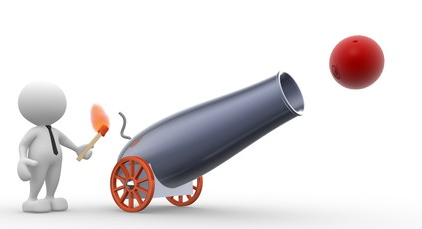
\includegraphics[scale=1]{cannon.png}
\end{figure}
\vfill
Manon Bruno, Julien Bricka, Romain Blondel\\
1M8, Gymnase Auguste Piccard\\
\today
\end{center}
\end{titlepage}

\tableofcontents
\thispagestyle{empty}
\clearpage

\setcounter{page}{1}

\section{But}
Déterminer la vitesse des balles à la sortie du canon  via les formules de la balistique.

\section{Introduction}
Comme dit juste au-dessus, les formules qui vont être utilisées sont celles de la balistique ainsi que de simples conversions d'unités ($[^{\circ}]$ en $[rad]$, $[cm]$ en $[m]$). La balistique se fonde sur la théorie du mouvement rectiligne uniformément accéléré (MRUA) ainsi que sa version "simplifiée" le mouvement rectiligne uniforme (MRU) :
\begin{itemize}
	\item[•] MRUA
	\begin{itemize}
		\item $a = constante$
		\item $v(t) = v_0 + a \cdot t$
		\item $x(t) = x_0 + v_0 \cdot t + \frac{1}{2} \cdot a \cdot t^2$
	\end{itemize}
	
	\item[•] MRU : MRUA à accélération nulle.
	\begin{itemize}
		\item $v = constante$
		\item $x(t) = x_0 + v_0 \cdot t$
	\end{itemize}
\end{itemize}
Où $a$ est l'accélération en $\left[\frac{m}{s^2}\right]$, $v$ ou $v(t)$ est la vitesse en $\left[\frac{m}{s}\right]$, $x$ ou $x(t)$ est la position en $[m]$ et $t$ le temps en $[s]$ ; si rien n'est précisé, les valeurs sont pour l'instant $t$, et $x_0$ ainsi que $v_0$ sont pour $t=0$.\\
La balistique est une décomposition du mouvement d'une balle sur deux dimension : horizontalement, il y a un MRU et verticalement, un MRUA avec une accélération valant celle de la gravitation terrestre et opposée à la montée, soit $a=-g\approx-9.81\left[\frac{m}{s^2}\right]$. Pour $v_0$ pour chaque direction, il suffit de séparer la vitesse initiale à l'aide des formules trigonométriques et de l'angle de départ. Voici les formules concrètes :
\begin{itemize}
\item $v_y (t) = v_{0y} - g \cdot t$
\item $y(t) = y_0 + v_{0y} \cdot t - \frac{1}{2} \cdot g \cdot t^2$
\item $x(t) = x_0 + v_{0x} \cdot t$
\item $v_{0y} = v_0 \cdot sin(\alpha)$
\item $v_{0x} = v_0 \cdot cos(\alpha)$
\end{itemize} 
Voilà toutes les formules utilisées dans la suite. 
\begin{figure}[H]
\centering
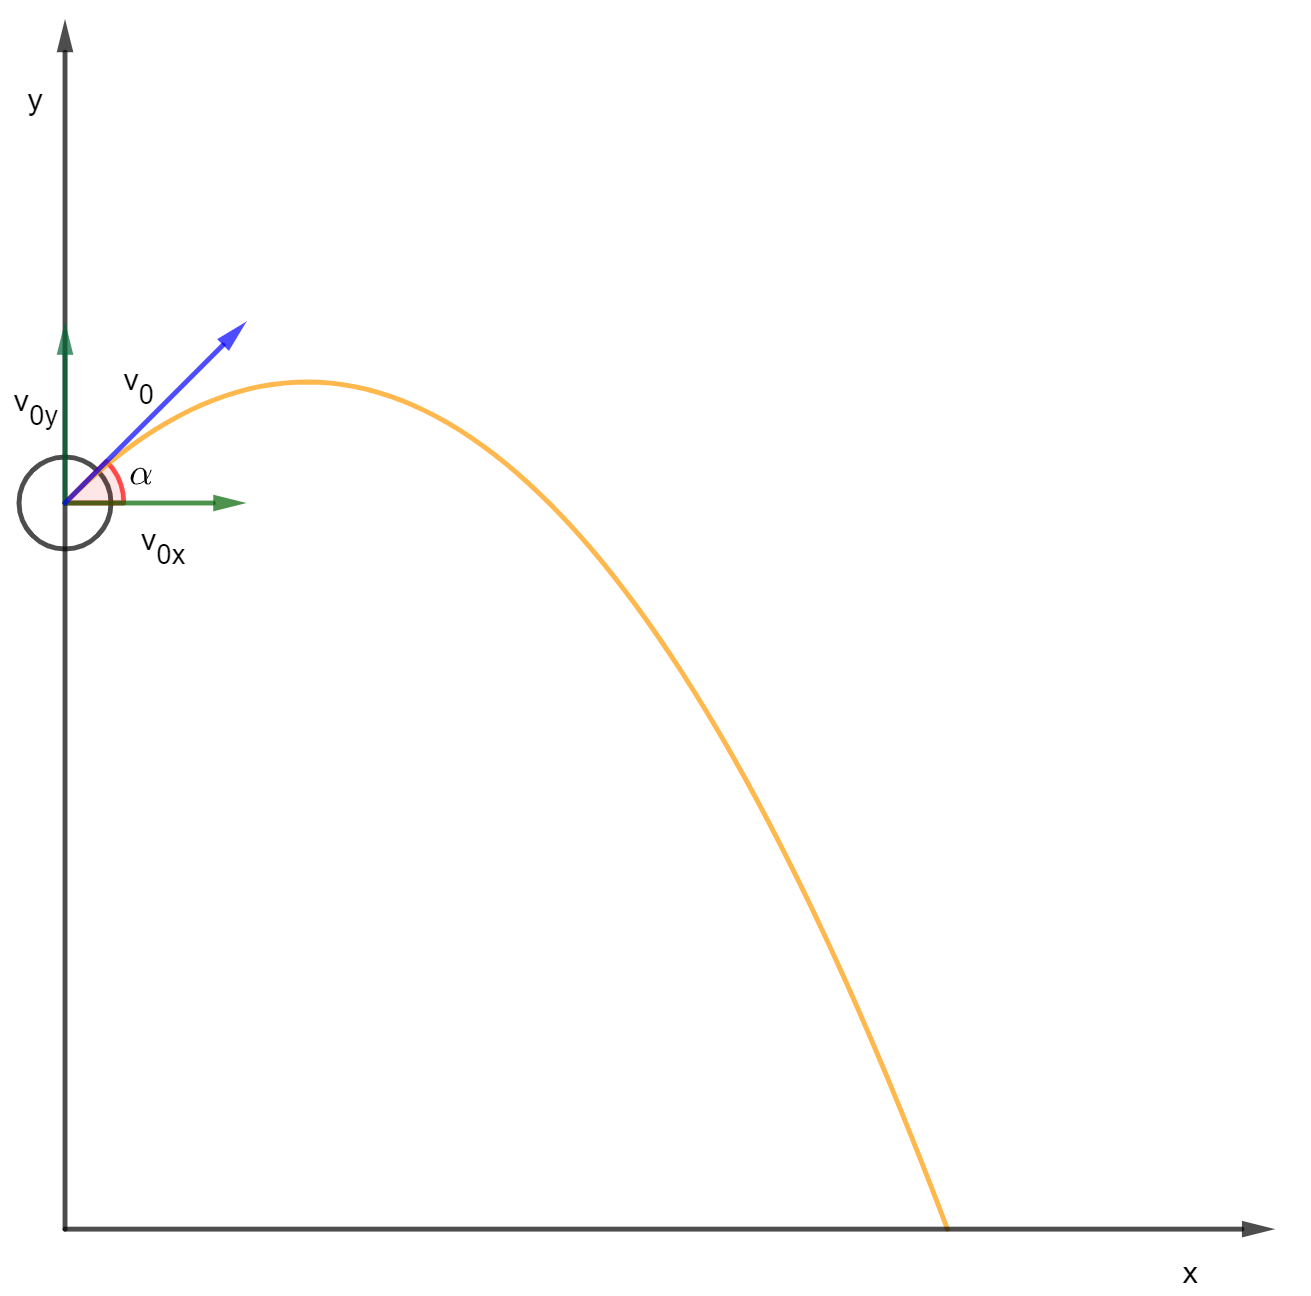
\includegraphics[scale=1.3]{geogebra-export.png}
\caption{Illustration d'un modèle de balistique}
\end{figure}
\clearpage

\section{Démarche}
\subsection{Matériel}
\subsubsection*{Pour l'expérience}
\begin{itemize}
\item[•] Canon
\item[•] Statif
\item[•] Fil à plomb
\item[•] Manchon
\item[•] Balle (en plastique)
\end{itemize} 

\subsubsection*{Pour la mesure}
\begin{itemize}
\item[•] Scotch (de carrossier)
\item[•] Mètre
\item[•] Stylo
\end{itemize}

\subsection{Marche à suivre}
\begin{enumerate}
\item Placer le lanceur aussi bien que possible sur un repère marqué afin de pouvoir mesurer les distances. 
\item Mesurer la hauteur entre le bout du canon et le sol ($y_0 = 26 [cm] = 0.26[m]$), ainsi que tout autre distance fixe (p.ex. du bout du canon à celui du socle, ...).
\item Régler l’angle de tire du canon a l’aide du fil à plomb, puis charger le projectile avec le manchon jusqu'au cran désiré.
\item Expulser le projectile en tirant sèchement sur la cordelette.
\item Marquer le lieu d’impact en y mettant un bout de scotch (\textit{note : annoter le scotch pour faciliter la mesure}).
\item  Mesurer les distances entre le lanceur et l’endroit où la balle a atterri.
\item Répéter l'opération en changeant les paramètres (\textit{cran du canon, angle}). 
\end{enumerate}

\subsection{Schéma du montage}
\begin{center}
\begin{figure}[H]
  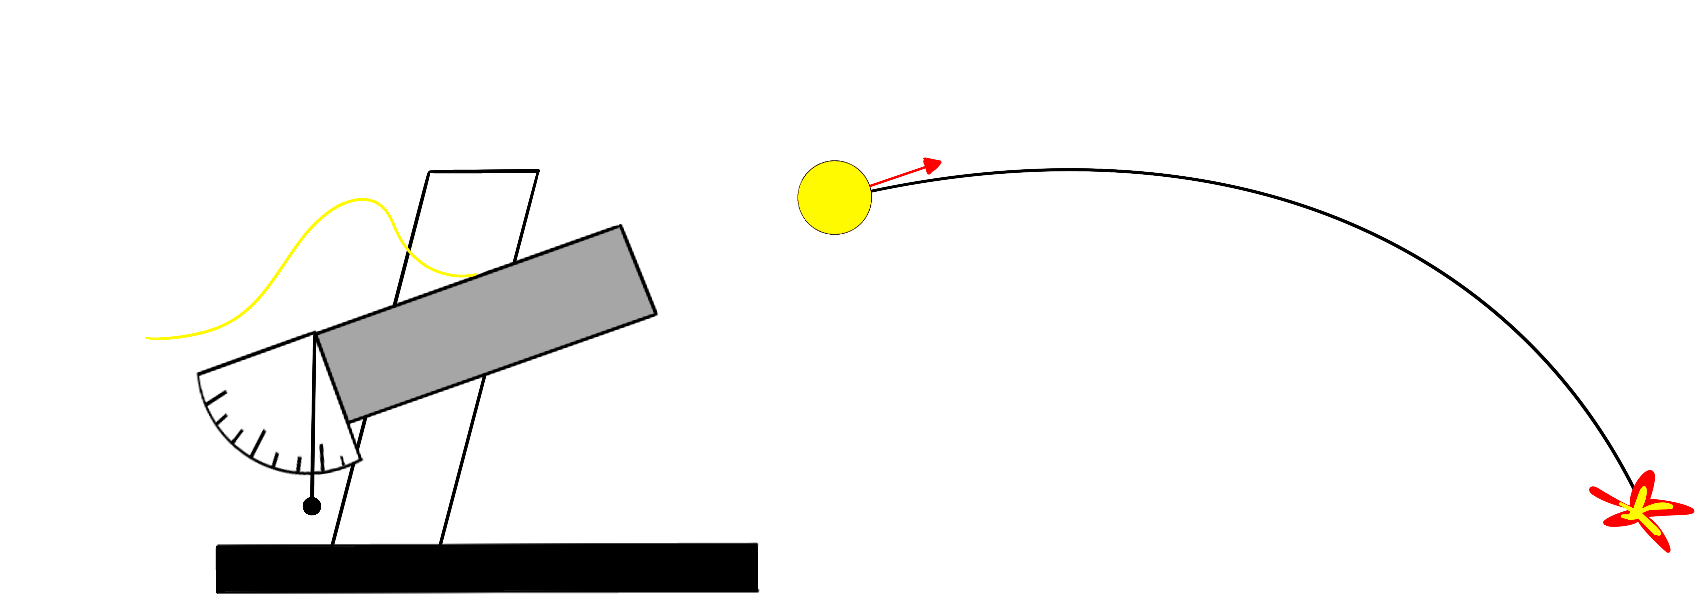
\includegraphics[scale=1]{schema.png}
  \caption{Schéma de l'expérience}
\end{figure}
\end{center}



\section{Résultats}
\subsection{Tableaux}
	\begin{table}[H]
		\centering
		\caption{Mesure d'angle ($\alpha$) et de distance ($x(t)$) pour chaque cran}	
		\label{fig:ang1}
		\begin{tabular}{ |>{\columncolor{lightgray}} l | l |>{\columncolor{lightgray}} l | l |>{\columncolor{lightgray}} l |}
			\hline
			\rowcolor{gray} mesure n° & angle $[^{\circ}]$ & cran 1 $[cm]$ & cran 2 $[cm]$ & cran 3 $[cm]$ \\ \hline
			1 & 30.00 & 109.50 & 227.50 & 425.00  \\ \hline 
			2 & 45.00 & 112.00 & 251.00 & 454.00  \\ \hline 
			3 & 60.00 & 88.00 & 215.00 & 383.00  \\ \hline 
		\end{tabular}
	\end{table}
	 
	\begin{table}[H]

		\centering
		\caption{Mesure d'angle et de distance en unité du système international}	
		\label{fig:ang2}	 
    	\begin{tabular}{ |>{\columncolor{lightgray}} l | l |>{\columncolor{lightgray}} l | l |>{\columncolor{lightgray}} l |}
			\hline
			\rowcolor{gray} mesure n° & angle $[rad]$ & cran 1 $[m]$ & cran 2 $[m]$ & cran 3 $[m]$ \\ \hline
			1 & 0.52 & 1.09 & 2.27 & 4.25  \\ \hline 
			2 & 0.79 & 1.12 & 2.51 & 4.54  \\ \hline 
			3 & 1.05 & 0.88 & 2.15 & 3.83  \\ \hline 
		\end{tabular}				
	\end{table}
	
	\begin{table}[H]
		\centering
		\caption{$v_0$ pour chaque cran}	 
    	\begin{tabular}{ |>{\columncolor{lightgray}} l | l |>{\columncolor{lightgray}} l | l |}
			\hline
			\rowcolor{gray} mesure n° & $v_0$ au cran 1 $\left[ \dfrac{m}{s} \right]$ & $v_0$ au cran 2 $\left[ \dfrac{m}{s} \right]$ & $v_0$ au cran 3 $\left[ \dfrac{m}{s} \right]$\\ \hline
			1 & 2.96 & 4.64 & 6.60  \\ \hline 
			2 & 2.99 & 4.72 & 6.49  \\ \hline 
			3 & 2.92 & 4.77 & 6.46  \\ \hline 
			Moyenne & 2.96 & 4.71 & 6.52  \\ \hline 
		\end{tabular}				
		\label{fig:v0}
	\end{table}
	
	\begin{table}[H]
		\centering
		\caption{$t_{final}$ pour chaque cran}	 
    	\begin{tabular}{ |>{\columncolor{lightgray}} l | l |>{\columncolor{lightgray}} l | l |}
			\hline
			\rowcolor{gray} mesure n° & $t_f$ au cran 1 $\left[ s \right]$ & $t_f$ au cran 2 $\left[ s \right]$ & $t_f$ au cran 3 $\left[ s \right]$\\ \hline
		1 & 0.43 & 0.57 & 0.74  \\ \hline 
		2 & 0.53 & 0.75 & 0.99  \\ \hline 
		3 & 0.60 & 0.90 & 1.19  \\ \hline 
		\end{tabular}	
		\label{fig:tf}			
	\end{table}
	
		\begin{table}[H]
		\centering
		\caption{Flèche pour chaque cran}	 
    	\begin{tabular}{ |>{\columncolor{lightgray}} l | l |>{\columncolor{lightgray}} l | l |}
			\hline
			\rowcolor{gray} mesure n° & $f$ au cran 1 $\left[ m \right]$ & $f$ au cran 2 $\left[ m \right]$ & $f$ au cran 3 $\left[ m \right]$\\ \hline
			1 & 0.37 & 0.53 & 0.81  \\ \hline 
			2 & 0.49 & 0.83 & 1.33  \\ \hline 
			3 & 0.59 & 1.13 & 1.86  \\ \hline  
		\end{tabular}
		\label{fig:fleche}				
	\end{table}
\textit{Note : les formules utilisées pour obtenir $v_0$, $t_{final}$ et les flèches seront développées dans la section suivante.}

\subsection{Graphiques}
\begin{center}
\begin{figure}[H] 
  \caption{Trajectoires théoriques de la balle à chaque cran}					
  \centering
  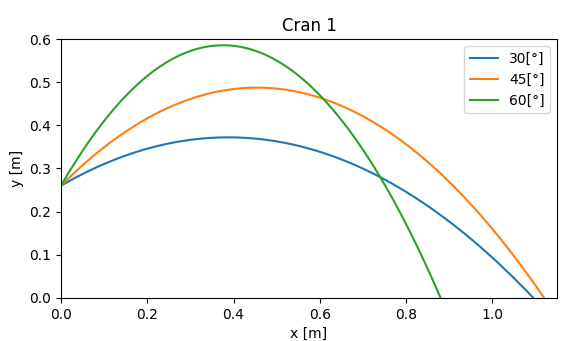
\includegraphics[scale=0.75]{graph1.png}
  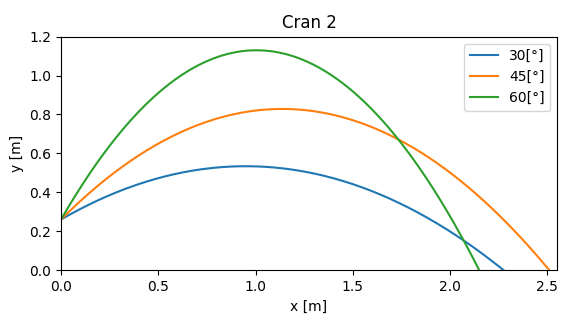
\includegraphics[scale=0.75]{graph2.png}
  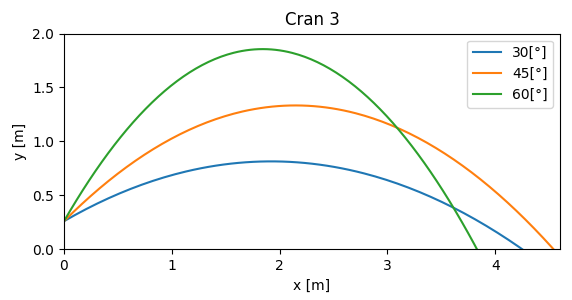
\includegraphics[scale=0.75]{graph3.png}
  \label{fig:traj}
\end{figure}
\end{center}
\textit{Note : les graphes ci-dessus sont faits via les résultats obtenus précédemment en se basant toujours sur la balistique et demeurent de fait très théoriques, ne prenant pas en compte de nombreux paramètres.}
	
	
\clearpage	
	
\section{Analyse des Résultats}
\subsection*{Comment trouver $v_0$ ?}
À partir de ce que l'on connait ($x(t)$, $\alpha$, $y_0$), et en tenant compte de ce que l'on ne connait pas ($t$), comment manipuler les formule de balistique pour obtenir une formule pour $v_0$ (cf. Table \ref{fig:v0})(\textit{note : le calcul est fait au moment où la balle touche le sol, soit avec $y(t) = 0$ et $x_0$ nulle}) :
$$x(t) = x_0 + v_{0x} \cdot t = v_{0x} \cdot t \Leftrightarrow t = \frac{x(t)}{v_{0x}}$$
$$y(t) =  y_0 + v_{0y} \cdot t - \frac{1}{2} \cdot g \cdot t^2 \Leftrightarrow 0 =  y_0 + v_{0y} \cdot \frac{x(t)}{v_{0x}} - \frac{1}{2} \cdot g \cdot \left(\frac{x(t)}{v_{0x}}\right)^2 =$$$$= y_0 + v_0 \cdot sin\alpha \cdot \frac{x(t)}{v_0 \cdot cos\alpha} - \frac{1}{2} \cdot g \cdot \frac{x(t)^2}{(v_0 \cdot cos\alpha)^2} = y_0 + x(t) \cdot tan\alpha - \frac{g \cdot x(t)^2}{2 \cdot v_0^2 \cdot cos^2\alpha} $$$$\Leftrightarrow \frac{g \cdot x(t)^2}{2 \cdot v_0^2 \cdot cos^2\alpha} = y_0 + x(t) \cdot tan\alpha \Leftrightarrow \frac{2 \cdot v_0^2 \cdot cos^2\alpha}{g \cdot x(t)^2}= \frac{1}{y_0 + x(t) \cdot tan\alpha}$$$$\Leftrightarrow v_0^2 = \frac{g \cdot x(t)^2}{2 \cdot cos^2\alpha \cdot (y_0 + x(t) \cdot tan\alpha)} \Leftrightarrow v_0 = \sqrt{\frac{g \cdot x(t)^2}{2 \cdot cos^2\alpha \cdot (y_0 + x(t) \cdot tan\alpha)}} $$
\subsection*{Que peut-on en faire ?}
Avec $v_0$, on a tout les paramètres pour établir les équations horaires des projectiles. De celle-ci, on peut faire des graphes de la trajectoire théorique des balles (cf. Figure \ref{fig:traj}), ainsi que pour n'importe quel autre angle ; obtenir le temps de vol de la balle  via $t = \frac{x(t)}{v_{0x}} \Leftrightarrow t = \frac{x(t)}{v_0 \cdot cos\alpha}$ (cf. Table \ref{fig:tf}) ; la flèche (point le plus haut) de la trajectoire de la balle : quand $v_y(t) = 0$, soit $v_y(t) = 0 = v_{0y} - g \cdot t \Leftrightarrow v_{0y} = g \cdot t \Leftrightarrow t = \frac{v_{0y}}{g}$, donc $f = y\left(\frac{v_{0y}}{g}\right) = y_0 + v_{0y} \cdot \frac{v_{0y}}{g} - \frac{1}{2} \cdot g \cdot \left(\frac{v_{0y}}{g}\right)^2 = y_0 + \frac{v_{0y}^2}{g} - \frac{1}{2} \cdot \frac{v_{0y}^2}{g} = y_0 + \frac{1}{2} \cdot \frac{v_{0y}^2}{g} = y_0 + \frac{v_0^2 \cdot sin^2\alpha}{2 \cdot g}$(cf. Table \ref{fig:fleche}).

\section{Conclusion}
En conclusion, l’expérience s’est bien passée mais manque énormément de précision au moment où il faut déterminer l’endroit où a atterri la balle ainsi qu’au moment des mesures au sol, le scotch étant large. Il serait donc possible d’améliorer la mesure à l’aide de marques plus fine ou d'une caméra. De plus, le modèle de la balistique omet certains paramètres comme les frottements de l'air, donc quelques mesures supplémentaires permettraient d'utiliser des calculs de force afin d'avoir des résultats plus réalistes.  

\clearpage

\end{document}